\documentclass[11pt,a4paper]{article}

\usepackage[margin=1in]{geometry}
\usepackage[T1]{fontenc}
\usepackage[utf8]{inputenc}
\usepackage{lmodern}
\usepackage{microtype}
\usepackage{graphicx}
\usepackage{booktabs}
\usepackage{array}
\usepackage{url}
\usepackage{hyperref}
\usepackage{amsmath,amssymb}
\usepackage{caption}
\usepackage{enumitem}
\usepackage{float}
\usepackage{xcolor}

\hypersetup{colorlinks=true,linkcolor=black,citecolor=black,urlcolor=blue}
\setlist[itemize]{leftmargin=1.5em}
\setlist[enumerate]{leftmargin=1.5em}
\captionsetup{font=small,labelfont=bf}

\title{An Experimental Comparison of Sorting Algorithms by Running-Time Measurement on Structured Inputs}
\author{Chircu Alexandru Cosmin\\Department of Computer Science\\West University of Timisoara\\\texttt{alexandru.chircu06@e-uvt.ro}}
\date{}

\begin{document}
\maketitle

\begin{abstract}
Sorting is a classical problem in algorithm design, but the fastest algorithm in practice depends on input size, input structure, element type, constant factors, implementation language, and memory behaviour. This paper reports an experimental comparison of sixteen sorting algorithms: elementary comparison sorts, divide-and-conquer methods, heap-based sorting, distribution-based sorting, adaptive and hybrid sorting, and a simple parallel merge sort. The experimental design measures repeated executions over integer, floating-point, and string inputs, using random, sorted, reverse-sorted, almost-sorted, half-sorted, and low-cardinality structures.

The measurements confirm the standard asymptotic separation between quadratic algorithms and $O(n\log n)$ algorithms, but they also show that asymptotic complexity alone is not sufficient for practical algorithm selection. Python's built-in Timsort is consistently the fastest method in the experiments, especially on already structured data. Distribution-based methods are competitive only under suitable assumptions on the key domain. Parallel merge sort helps only for sufficiently large inputs and remains limited by process-management and merging overhead. The code and raw results are made available with this paper so that the experiment can be reproduced, checked, and extended.
\end{abstract}

\section{Introduction}

Sorting transforms a sequence of comparable elements into nondecreasing order. It is one of the standard problems studied in an introductory algorithms course because it offers simple algorithms such as insertion sort, classical divide-and-conquer algorithms such as merge sort and quicksort, lower-bound results for comparison sorting, and linear-time algorithms under additional assumptions about the keys. At the same time, sorting is not only a theoretical exercise. It is used inside databases, file systems, search engines, programming-language libraries, and data-analysis pipelines. A difference of a few constant factors in sorting performance may be insignificant for twenty elements but relevant for one million elements.

The purpose of this paper is to compare sorting algorithms experimentally, not only by restating their known worst-case complexities. The study includes algorithms usually covered in an Algorithms lecture: bubble sort, selection sort, insertion sort, merge sort, quicksort, heap sort, counting sort, radix sort, bucket sort, and shell sort. It also includes additional algorithms that are important in practice or useful as comparison points: Timsort, introsort, iterative merge sort, comb sort, patience sort, and parallel merge sort. Standard algorithmic notation and complexity terminology are used in the sense of common algorithm textbooks such as Cormen et al.~\cite{cormen2009} and Knuth~\cite{knuth1998}.

The central question is the following: when the same benchmark framework is used, how do different sorting algorithms behave as the input size, input structure, and element type change? The answer is not expected to be one universal winner. For example, insertion sort has quadratic worst-case complexity but is often efficient on small or nearly sorted inputs. Counting sort and radix sort can run in linear or near-linear time, but only when the key representation and range make them applicable. Timsort is adaptive and exploits monotone runs in the data, which makes it particularly effective on data that is already sorted or partly sorted.

The contribution of this paper is an original experimental study and a reproducible artifact. I implemented or used sixteen sorting procedures in a single Python benchmark, generated a systematic test matrix, recorded raw measurements in CSV format, and interpreted the results against the theoretical properties of the algorithms. This contribution is experimental and comparative: the algorithms themselves are known, but the paper gives a concrete, reproducible analysis of their behaviour under one implementation model.

The paper follows the structure expected for the MPI paper standard. Section~\ref{sec:formal} gives a formal description of the sorting problem and of the main algorithm families. Section~\ref{sec:implementation} describes the computational model, implementation, and artifact. Section~\ref{sec:experiment} presents the experimental design and results. Section~\ref{sec:related} places the work in relation to previous research. Section~\ref{sec:conclusion} summarizes the findings and limitations.

\section{The Sorting Problem and Algorithmic Families}\label{sec:formal}

\subsection{Problem statement}

Let $A=\langle a_1,a_2,\ldots,a_n\rangle$ be a finite sequence of elements from a domain $D$ equipped with a total preorder $\leq$. The sorting problem asks for a permutation $\pi$ of $\{1,2,\ldots,n\}$ such that
\[
 a_{\pi(1)} \leq a_{\pi(2)} \leq \cdots \leq a_{\pi(n)}.
\]
A sorting algorithm is correct if, for every valid input sequence, it returns a sequence that is ordered and contains exactly the same multiset of elements as the input. The first condition is sortedness; the second condition is preservation of elements. In this paper, the benchmark checks correctness by comparing each algorithm's output with the output of Python's reference sorting operation on small random inputs before timing begins.

There are two broad theoretical classes relevant to the experiment. Comparison sorts obtain information only by comparing elements. Their decision-tree lower bound implies that every comparison sort needs $\Omega(n\log n)$ comparisons in the worst case. Non-comparison or distribution-based sorts use information about the representation of keys, such as integer digits or integer ranges; under suitable assumptions they can achieve linear or near-linear time in the number of elements and the size of the key representation~\cite{cormen2009,knuth1998}.

\subsection{Algorithms included in the comparison}

Table~\ref{tab:algorithms} summarizes the algorithms included in the experiment. The complexities are the usual high-level theoretical values; they are not exact predictions for the Python implementation. In particular, the built-in Timsort is implemented in optimized C, while most other algorithms in the benchmark are implemented directly in Python. This is not a defect of the experiment, but it must be considered when interpreting the constant factors.

\begin{table}[H]
\centering
\caption{Algorithms compared in the experiment.}
\label{tab:algorithms}
\small
\begin{tabular}{p{0.22\linewidth}p{0.31\linewidth}p{0.23\linewidth}p{0.14\linewidth}}
\toprule
Algorithm & Main idea & Typical time complexity & Extra assumptions \\
\midrule
Bubble sort & Repeated adjacent swaps & $O(n^2)$ worst case & None \\
Selection sort & Repeatedly select minimum & $O(n^2)$ & None \\
Insertion sort & Insert each item into sorted prefix & $O(n^2)$, $O(n)$ best case & None \\
Merge sort & Divide, sort halves, merge & $O(n\log n)$ & None \\
Quicksort & Partition around a pivot & Average $O(n\log n)$, worst $O(n^2)$ & Pivot quality matters \\
Heap sort & Use binary heap selection & $O(n\log n)$ & None \\
Counting sort & Count key frequencies & $O(n+k)$ & Integer range $k$ manageable \\
Radix sort & Sort by digits from least significant digit & $O(d(n+b))$ & Digit representation \\
Bucket sort & Scatter into buckets and sort buckets & Expected linear under distribution assumptions & Numeric keys \\
Shell sort & Gapped insertion sorting & Gap-dependent & None \\
Timsort & Adaptive merge sort using runs & $O(n\log n)$ worst case, adaptive on runs & None \\
Introsort & Quicksort with depth limit and heapsort fallback & $O(n\log n)$ worst case & None \\
Iterative merge sort & Bottom-up merging & $O(n\log n)$ & None \\
Comb sort & Bubble-sort variant with shrinking gaps & Usually better than bubble sort & None \\
Patience sort & Builds piles and performs heap merge & $O(n\log n)$ & None \\
Parallel merge sort & Sort chunks in parallel and merge & Work $O(n\log n)$ plus overhead & Multiple cores \\
\bottomrule
\end{tabular}
\end{table}

The elementary algorithms are included because they are pedagogically important. Bubble sort, selection sort, and insertion sort make the cost of nested loops visible. Merge sort and heap sort represent guaranteed $O(n\log n)$ comparison sorting. Quicksort, originally introduced by Hoare~\cite{hoare1962}, is a central example of an algorithm with strong average performance but sensitive worst-case behaviour. Heap sort comes from Williams' heap data structure~\cite{williams1964}. Shell sort, introduced by Shell~\cite{shell1959}, illustrates how a simple idea can improve insertion sort by moving elements over larger gaps before final local cleanup.

The additional algorithms are included to connect lecture material with modern practice. Timsort was designed for real-world partially ordered data and is used by Python's sorting routine~\cite{peters2002}. Introsort, proposed by Musser~\cite{musser1997}, combines the average-case speed of quicksort with a worst-case guarantee by switching strategy when recursion becomes too deep. Parallel merge sort is included because parallel sorting is a classical research topic~\cite{hirschberg1978}, although the implementation used here is intentionally simple and uses Python processes rather than specialized parallel hardware.

\section{Implementation Model and Reproducibility}\label{sec:implementation}

\subsection{Computational model}

The benchmark is implemented in Python. Each sorting function receives a list and returns a sorted list. To avoid modifying the input shared across repetitions, the algorithms copy the array internally before sorting, except where the algorithm is naturally expressed recursively and creates new lists. The benchmark measures wall-clock elapsed time using \texttt{time.perf\_counter}. Garbage collection is disabled during a single timed call and re-enabled immediately afterward. This reduces one source of timing noise, although it does not eliminate all operating-system and interpreter effects.

The dataset generator uses a fixed random seed to make the experiments reproducible. The generated values cover three element types: integers, floating-point numbers, and strings. The generated structures are random, sorted, reverse-sorted, almost-sorted, half-sorted, and flat. The flat structure is meaningful mainly for integers, where it uses only five distinct values. The benchmark therefore makes it possible to observe both scale effects and structural effects.

\subsection{Artifact availability}

The experimental artifact consists of two files: \texttt{Experimental\_analysis\_sort.py}, containing the benchmark and the algorithm implementations, and \texttt{results.csv}, containing the raw measurements. For public submission, these files should be placed in a repository such as:
\[
\texttt{https://github.com/alexandruchircuDex/Experimental\_sorting\_algorithms\_example}
\]
The present submission package already includes the same files next to this paper. A reproducible repository should contain the following structure:

\begin{verbatim}
sorting-algorithms-experiment/
  src/Experimental_analysis_sort.py
  data/results.csv
  paper/sorting_algorithms_experimental_comparison.tex
  paper/figures/
  README.md
\end{verbatim}

A full run can be started with:

\begin{verbatim}
python3 Experimental_analysis_sort.py --output results.csv
\end{verbatim}

A faster smoke test can be started with:

\begin{verbatim}
python3 Experimental_analysis_sort.py --quick --output quick_results.csv
\end{verbatim}

The code first runs a correctness check on all non-parallel algorithms using small random integer inputs. The results file stores the algorithm name, input size, input structure, element type, number of repetitions, mean time, minimum time, and maximum time. This is sufficient to reproduce the figures and tables in this paper. A limitation is that the CSV file does not store hardware, operating-system, Python-version, or CPU-load metadata. Therefore, the exact numerical values should be interpreted as measurements from one execution environment, while the trends are more important than the absolute milliseconds.

\section{Experimental Design and Results}\label{sec:experiment}

\subsection{Design of the experiment}

The experiment uses a factorial design over algorithms, input sizes, input structures, and element types. The integer input sizes range from $20$ to $1,000,000$. Floating-point and string tests stop at $100,000$ elements in the available results. The benchmark repeats smaller runs many times and larger runs fewer times: for example, inputs of size at most $50$ use $500$ repetitions, while very large inputs use one repetition. This design reduces noise for fast executions and keeps the total running time feasible.

Some algorithms are skipped in cases where they are not applicable or would be impractically slow. Counting sort and radix sort are used only for non-negative integers. Bucket sort is used only for numeric values. Bubble sort, selection sort, and insertion sort are limited to $n\leq 5000$, because their quadratic growth would otherwise dominate the benchmark time. Parallel merge sort is skipped below $n=10000$, because process-creation and communication overhead are not worthwhile for small inputs.

\subsection{Overall scaling on random integer inputs}

Figure~\ref{fig:random-int} shows the performance of scalable algorithms on random integer inputs. The vertical and horizontal axes use logarithmic scales. The main result is that Timsort dominates the tested implementations. At $n=1,000,000$ random integers, the mean time for Timsort is $304.27$ ms, compared with $892.01$ ms for parallel merge sort, $1105.05$ ms for bucket sort, $2652.94$ ms for counting sort, and $4514.75$ ms for radix sort. The result is not surprising in Python: Timsort is implemented as optimized library code, while most competing algorithms are Python-level implementations.

\begin{figure}[H]
\centering
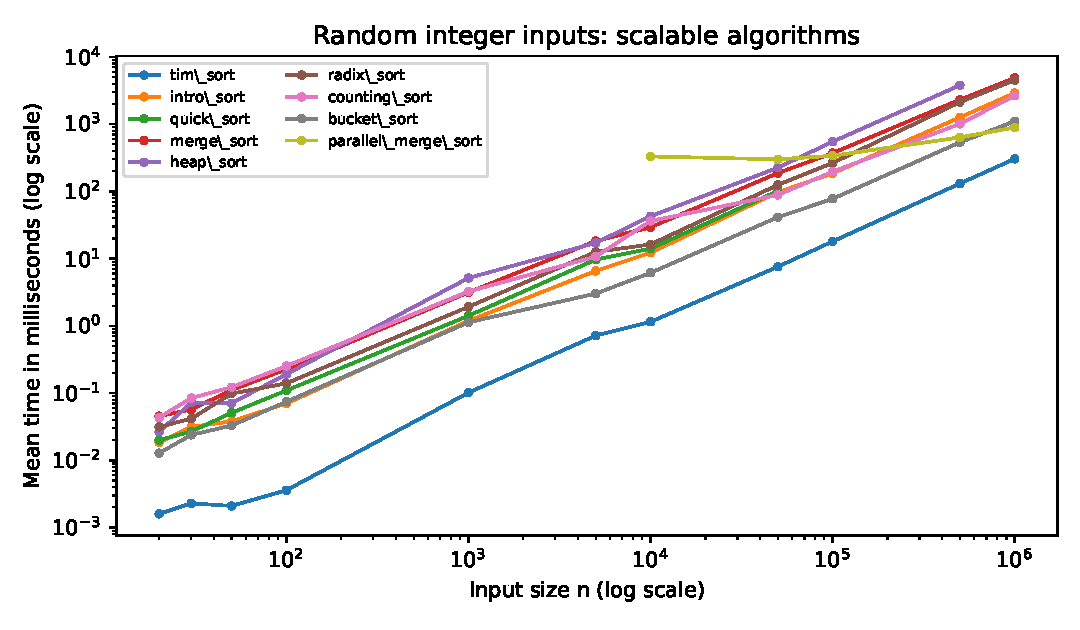
\includegraphics[width=0.88\linewidth]{figures/random_int_scalable.pdf}
\caption{Running time on random integer inputs for scalable algorithms. Both axes use logarithmic scale.}
\label{fig:random-int}
\end{figure}

The data also show that theoretical linear-time methods are not automatically fastest in a high-level implementation. Counting sort must allocate and fill a count array whose size depends on the key range. Radix sort performs several passes over the data. Bucket sort depends on the bucket distribution and then on the cost of sorting within buckets. These algorithms can be excellent under favorable low-level implementations and key assumptions, but in this benchmark their overhead is visible.

\subsection{Effect of input structure}

Figure~\ref{fig:timsort-structure} isolates Timsort and compares input structures on integer data. The difference is large. At $n=100,000$, Timsort takes approximately $18.01$ ms on random integers, $6.74$ ms on almost-sorted integers, $1.57$ ms on sorted integers, and $1.61$ ms on reverse-sorted integers. This is a practical demonstration of adaptivity: the algorithm can exploit long runs already present in the input.

\begin{figure}[H]
\centering
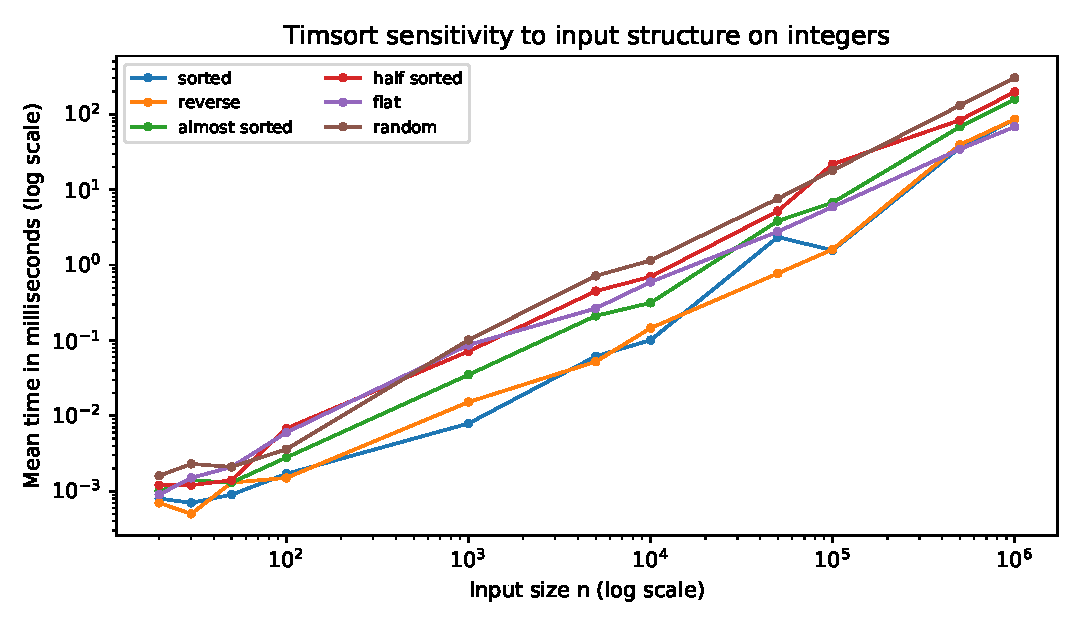
\includegraphics[width=0.88\linewidth]{figures/timsort_structure.pdf}
\caption{Timsort behaviour on different integer input structures. The algorithm benefits strongly from already ordered structure.}
\label{fig:timsort-structure}
\end{figure}

The flat integer case also illustrates why input distribution matters. At $n=100,000$ and five distinct integer values, counting sort takes $10.13$ ms, radix sort takes $38.15$ ms, bucket sort takes $52.23$ ms, and Timsort takes $5.91$ ms. Counting sort improves because the effective key range is small, but Timsort remains faster in this Python benchmark because its implementation is highly optimized and because repeated values produce simple comparisons and long runs after partial organization.

\subsection{Small inputs and elementary algorithms}

Figure~\ref{fig:quadratic} compares elementary and gap-based algorithms on random integer inputs up to the configured limit. The curve for bubble sort grows quickly. Selection sort and insertion sort are also quadratic in the random case, although insertion sort is usually more competitive for small inputs because it performs less unnecessary work. Comb sort and shell sort reduce the practical cost by moving elements over larger gaps, but they do not match the best $O(n\log n)$ methods at larger sizes.

\begin{figure}[H]
\centering
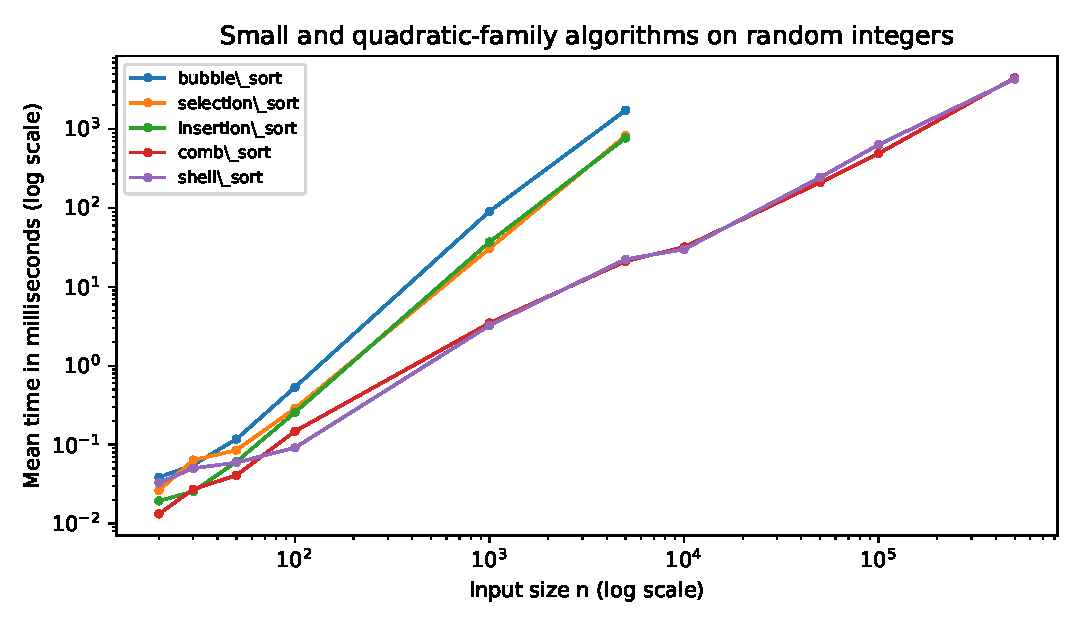
\includegraphics[width=0.88\linewidth]{figures/quadratic_algorithms.pdf}
\caption{Elementary and gap-based algorithms on random integer inputs. Quadratic behaviour becomes visible as $n$ increases.}
\label{fig:quadratic}
\end{figure}

For $n=100$ random integers, Timsort already has the best measured mean time ($0.0036$ ms). Among pure Python algorithms, introsort, bucket sort, shell sort, and quicksort are among the better performers. Bubble sort is slowest among the measured methods at this size. These small-input results are important because constant factors dominate; they should not be interpreted only through asymptotic notation.

\subsection{Element type comparison}

Table~\ref{tab:selected-results} reports selected winners on the largest random input available for each element type. For integers, the largest available size is $1,000,000$; for floats and strings, it is $100,000$. Timsort is the fastest in all three categories. The relative order after Timsort changes with element type. Bucket sort is strong on numeric data, while quicksort, patience sort, and introsort are competitive on strings.

\begin{table}[H]
\centering
\caption{Five fastest algorithms on the largest random input available for each element type. Times are mean milliseconds.}
\label{tab:selected-results}
\small
\begin{tabular}{llrr}
\toprule
Element type & Algorithm & $n$ & Mean ms \\
\midrule
Integer & Timsort & 1,000,000 & 304.27 \\
Integer & Parallel merge sort & 1,000,000 & 892.01 \\
Integer & Bucket sort & 1,000,000 & 1105.05 \\
Integer & Counting sort & 1,000,000 & 2652.94 \\
Integer & Patience sort & 1,000,000 & 2679.21 \\
\midrule
Float & Timsort & 100,000 & 17.07 \\
Float & Bucket sort & 100,000 & 67.18 \\
Float & Quicksort & 100,000 & 178.77 \\
Float & Patience sort & 100,000 & 194.98 \\
Float & Introsort & 100,000 & 199.97 \\
\midrule
String & Timsort & 100,000 & 27.46 \\
String & Quicksort & 100,000 & 234.30 \\
String & Patience sort & 100,000 & 247.97 \\
String & Introsort & 100,000 & 248.08 \\
String & Parallel merge sort & 100,000 & 381.96 \\
\bottomrule
\end{tabular}
\end{table}

The string results are slower than integer comparisons in several algorithms because string comparison may inspect multiple characters before determining order. The benchmark uses fixed-length lowercase strings of length eight, which controls but does not remove this cost. The fact that Timsort remains very strong on strings is consistent with its optimized implementation and adaptive merge strategy.

\subsection{Threats to validity}

The main internal threat is implementation inequality. Timsort uses Python's built-in \texttt{sorted}, implemented in optimized C, while the other algorithms are written directly in Python. Therefore, the experiment compares practical available implementations rather than perfectly equal machine-code implementations of all algorithms. A second threat is environmental noise: CPU frequency scaling, background processes, cache state, and memory allocation can affect wall-clock timing. The benchmark reduces noise by using repetitions and fixed data generation, but it does not remove it entirely. A third threat is input representativeness. The generated structures are useful, but real datasets may contain domain-specific patterns not covered here.

These limitations do not invalidate the experiment. They define its scope. The paper answers how these implementations behave in this Python benchmark, not how all possible implementations would behave on all hardware. This distinction is important in experimental computer science: a reproducible benchmark is evidence, but it is evidence under a specified model.

\section{Related Work}\label{sec:related}

The theoretical background of sorting is well established. Knuth's treatment of sorting and searching~\cite{knuth1998} remains a central source for classical algorithms and historical context. Cormen et al.~\cite{cormen2009} provide the standard textbook presentation of comparison sorting, the decision-tree lower bound, heap sort, quicksort, counting sort, radix sort, and bucket sort. The present paper uses these sources for definitions and theoretical expectations, then checks how selected algorithms behave experimentally.

Several algorithms in the benchmark come from original research contributions. Hoare's quicksort~\cite{hoare1962} is included because it remains one of the most influential practical sorting algorithms. Williams' heap construction~\cite{williams1964} underlies heap sort. Shell's diminishing-increment method~\cite{shell1959} motivates shell sort. Musser's introspective sorting~\cite{musser1997} is directly relevant to hybrid design because it shows how an implementation can combine a fast average-case method with a worst-case safeguard.

The experiment also connects to research on adaptive and parallel sorting. Timsort, designed by Peters~\cite{peters2002}, is important because it was built for partially ordered real-world data rather than only for random input. Parallel sorting has a long history; Hirschberg~\cite{hirschberg1978} studied fast parallel sorting algorithms, and later manycore work such as Satish et al.~\cite{satish2009} shows that architecture-aware implementation can change practical conclusions. The parallel merge sort in this paper is much simpler than those systems, so its role is only to indicate the overheads and potential of parallelism in a Python multiprocessing model.

\section{Conclusions and Future Work}\label{sec:conclusion}

This paper experimentally compared sixteen sorting algorithms over a structured benchmark matrix. The results support the theoretical distinction between $O(n^2)$ and $O(n\log n)$ algorithms: bubble sort, selection sort, and insertion sort become impractical as input size grows. However, the results also show that practical performance cannot be predicted from asymptotic complexity alone. Constant factors, implementation language, memory allocation, input structure, and element type strongly influence running time.

The strongest empirical conclusion is that Timsort is the best practical choice in the tested Python environment. It is fast on random input and extremely fast on sorted, reverse-sorted, and almost-sorted input. Introsort, quicksort, merge sort, and heap sort behave consistently with their theoretical roles, but they are slowed by Python-level implementation overhead. Distribution-based algorithms are useful when their assumptions are satisfied, especially for small integer ranges, but they are not universal winners in this experiment. Parallel merge sort shows that parallelism introduces overhead and should be used only when the input size is large enough to compensate for it.

Future work should improve the experiment in four directions. First, the benchmark should store hardware and software metadata automatically. Second, the same algorithms should be implemented in a compiled language such as C++ or Rust to reduce interpreter effects. Third, additional real-world datasets should be used, for example log records, already clustered values, and strings with common prefixes. Fourth, memory consumption and cache behaviour should be measured alongside time. These extensions would make the comparison more complete and would separate algorithmic effects from implementation-language effects more clearly.

\begin{thebibliography}{99}

\bibitem{cormen2009}
Thomas H. Cormen, Charles E. Leiserson, Ronald L. Rivest, and Clifford Stein.
\newblock \emph{Introduction to Algorithms}.
\newblock 3rd edition, MIT Press, 2009.

\bibitem{hirschberg1978}
Daniel S. Hirschberg.
\newblock Fast parallel sorting algorithms.
\newblock \emph{Communications of the ACM}, 21(8):657--661, 1978.

\bibitem{hoare1962}
C. A. R. Hoare.
\newblock Quicksort.
\newblock \emph{The Computer Journal}, 5(1):10--16, 1962.

\bibitem{knuth1998}
Donald E. Knuth.
\newblock \emph{The Art of Computer Programming, Volume 3: Sorting and Searching}.
\newblock 2nd edition, Addison-Wesley, 1998.

\bibitem{musser1997}
David R. Musser.
\newblock Introspective sorting and selection algorithms.
\newblock \emph{Software: Practice and Experience}, 27(8):983--993, 1997.

\bibitem{peters2002}
Tim Peters.
\newblock Timsort description and implementation notes.
\newblock Python Software Foundation, 2002.

\bibitem{satish2009}
Nadathur Satish, Mark Harris, and Michael Garland.
\newblock Designing efficient sorting algorithms for manycore GPUs.
\newblock In \emph{2009 IEEE International Symposium on Parallel \& Distributed Processing}, pages 1--10. IEEE, 2009.

\bibitem{shell1959}
Donald L. Shell.
\newblock A high-speed sorting procedure.
\newblock \emph{Communications of the ACM}, 2(7):30--32, 1959.

\bibitem{williams1964}
J. W. J. Williams.
\newblock Algorithm 232: Heapsort.
\newblock \emph{Communications of the ACM}, 7(6):347--348, 1964.

\end{thebibliography}

\end{document}
